\documentclass[12pt]{article}
\usepackage{amsmath}
\usepackage{graphicx}
\usepackage{hyperref}
\usepackage[latin1]{inputenc}
\usepackage{listings}
\renewcommand{\labelitemi}{$\textendash$}

\title{CS3031: Project II}
\author{Conor McCauley - 17323203}
\date{April 13, 2020}

\begin{document}

\maketitle

\section{Implementation}

\subsection{Overview}

\indent The project consists of two primary components: a client application and a server. The server is implemented using a Flask API in Python. It stores information on active users, groups and encrypted messages and responds to HTTP requests from instances of the client application.

\indent The client application is also implemented in Python. It allows a user to login with a unique username and password and create or join messaging groups. From inside these groups the creator can add and remove participants while all members of the group can send messages.

\indent All API requests require authentication in the form of a password which is provided by the client and compared with the server's hashed version.

\subsection{Encryption}

\indent Each pair of users in a group share a unique RSA key pair. Whenever a user sends a message into the group it is encrypted separately for each other user in the group using the appropriate public key. Other users can sort through the different encrypted versions of the message and select the version intended for them and then decrypt it using the the appropriate private key.

\indent In order to exchange keys each client listens for requests on a unique port. Whenever a new user joins a group they receive a list of user ports from the API and, for each user, generates new RSA keys and sends the public key to that user via a socket. The other user then responds in the same manner. No further direct communication between the two users is required.

\indent The key exchange does not occur via the server meaning that only the two relevant users are aware of their key pairs. One improvement that could be made to the implementation would be to wrap all socket communications in SSL in order to prevent malevolent actors from eavesdropping on the client-to-client communication.

\indent In summary the communication between two clients follows the following structure:

\begin{enumerate}
  \item Client 1: joins group.
  \item Client 1: generates RSA keys for communication with client 2 and stores the private key locally.
  \item Client 1: sends the public key to client 2 via a socket.
  \item Client 2: receives the public key and stores it locally.
  \item Client 2: generates RSA keys for communication with client 1 and stores the private key locally.
  \item Client 2: sends the public key to client 1 via the same socket.
  \item Client 1: receives the public key and stores it locally.
  \item Both clients now have local public and private keys for decrypting and encrypting messages.
\end{enumerate}

\subsection{Examples}

\indent This section just contains a couple of screenshots of the messaging application being used.

\subsubsection{Console and GUI for Alice}

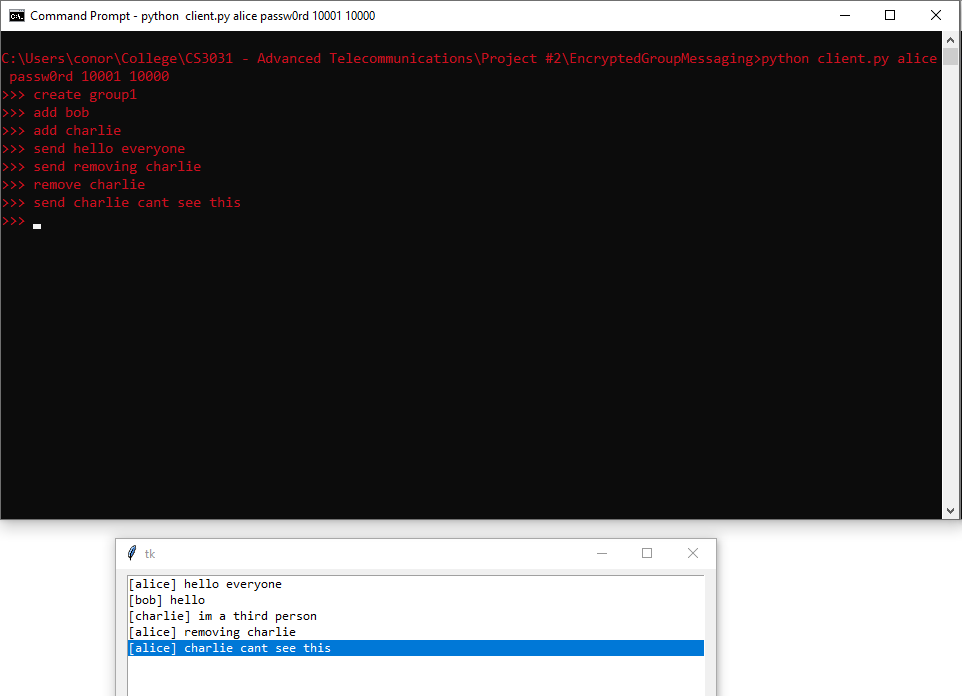
\includegraphics[scale=0.8]{alice_both.png}

\subsubsection{Console and GUI for Charlie}

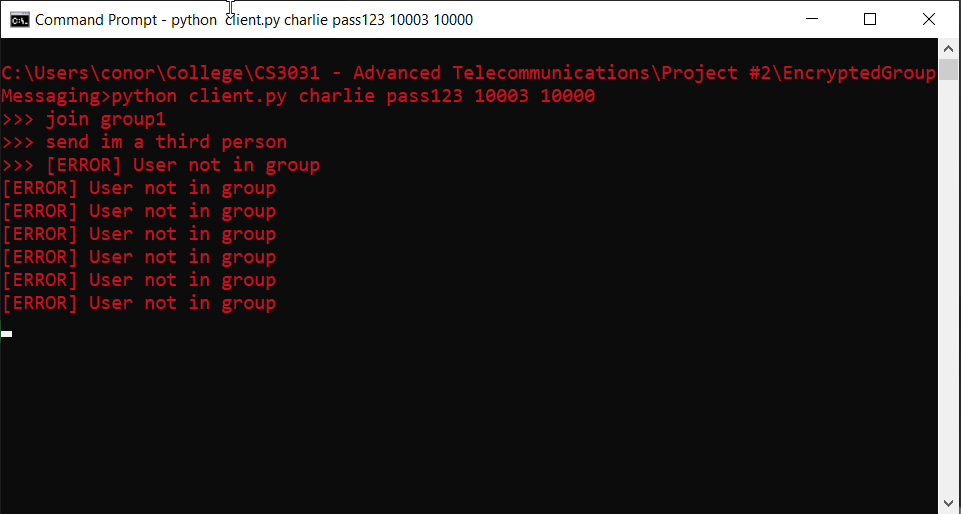
\includegraphics[scale=0.8]{charlie_console.png}

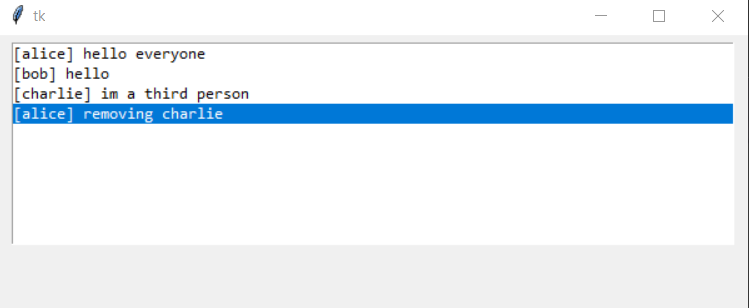
\includegraphics[scale=0.8]{charlie_gui.png}

\subsubsection{Server log for this example}

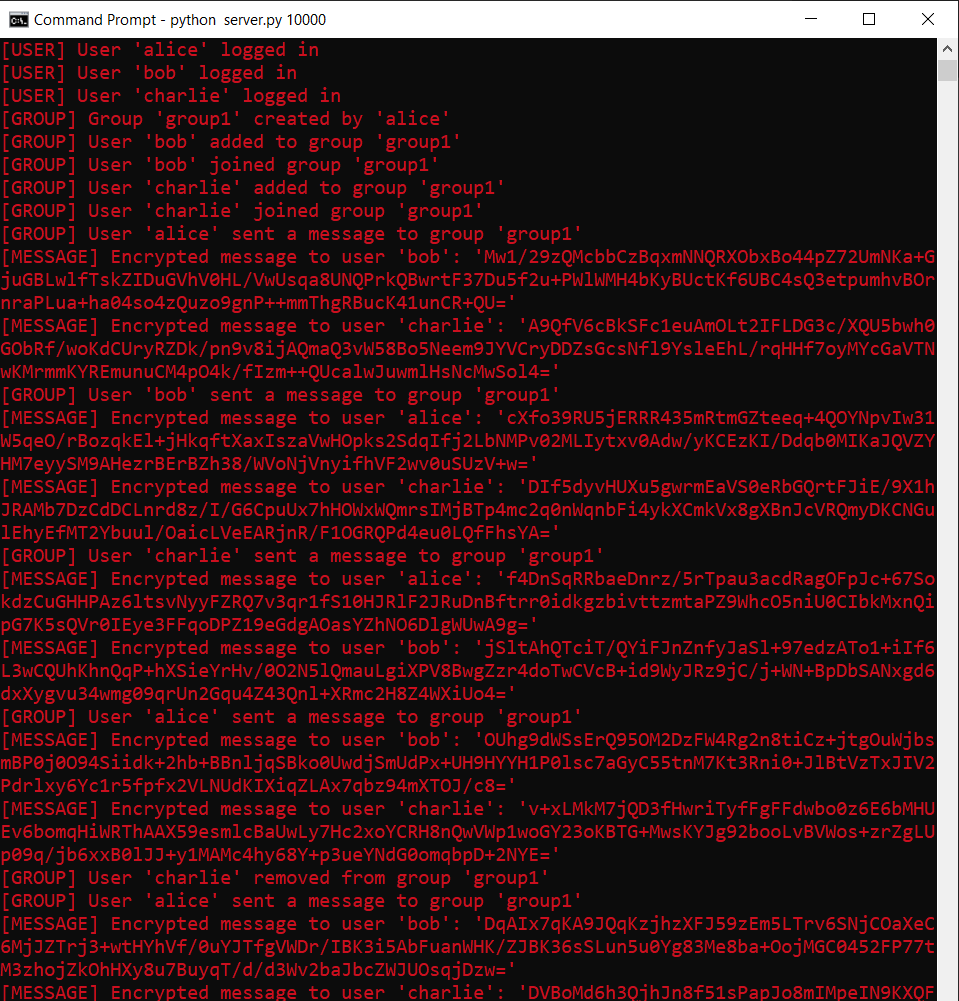
\includegraphics[scale=0.8]{server.png}

\section{Code Listing}

\subsection{Client}

\lstset{%
    language=Python,
    basicstyle=\footnotesize,
    breaklines=true
}
\lstinputlisting{client.py}

\subsection{Server}

\lstset{%
    language=Python,
    basicstyle=\footnotesize,
    breaklines=true
}
\lstinputlisting{server.py}

\end{document}
